% Real-time Face Recognition System: Quick Start and User Guide
% Style follows the AI VIET NAM course notes (serif body, green running header, Roman numbered
% sections, coloured call-out boxes and titled code listings).
% Build: tectonic USER_GUIDE.tex   (or xelatex USER_GUIDE.tex)
\documentclass[10pt,a4paper]{article}

\usepackage[a4paper,top=2.3cm,bottom=1.6cm,left=2cm,right=2cm,headheight=1.1cm,headsep=0.45cm]{geometry}
\usepackage{fontspec}          % Latin Modern (Computer Modern look) is the default
\usepackage{microtype}
\usepackage{graphicx}
\usepackage{xcolor}
\usepackage{fancyhdr}
\usepackage{titlesec}
\usepackage{enumitem}
\usepackage{caption}
\usepackage{tabularx}
\usepackage{fontawesome5}
\usepackage[skins,breakable,listings]{tcolorbox}
\usepackage{listings}
\usepackage[colorlinks=true,urlcolor=linkblue,linkcolor=linkblue]{hyperref}

% ---- palette taken from the AI VIET NAM notes -----------------------------------------------
\definecolor{aiogreen}{HTML}{3A5A27}
\definecolor{aiopurple}{HTML}{34388A}
\definecolor{linkblue}{HTML}{1F1FD6}
\definecolor{codekw}{HTML}{D6336C}
\definecolor{codecmt}{HTML}{1E8E1E}
\definecolor{codestr}{HTML}{C92A2A}
\definecolor{codefn}{HTML}{1C4FC4}
\definecolor{muted}{HTML}{666666}

\setlength{\parindent}{0pt}
\setlength{\parskip}{3pt}
\linespread{1.07}
\setlist{nosep,leftmargin=1.5em,itemsep=3pt,topsep=2pt}
\setlist[itemize,1]{label=\textbullet}

% ---- running header and footer ------------------------------------------------------------------
\pagestyle{fancy}
\fancyhf{}
\fancyhead[L]{\raisebox{-0.17cm}{
\includegraphics[height=0.7cm]{figures/tni_logo.png}}\hspace{0.6em}\textbf{\color{aiogreen}FACE RECOGNITION SYSTEM}}
\fancyhead[R]{\textbf{\color{aiogreen}TNI Tech}}
\fancyfoot[C]{\thepage}
\renewcommand{\headrulewidth}{0.9pt}
\renewcommand{\footrulewidth}{0pt}
\makeatletter
\def\headrule{{\color{aiogreen}\hrule\@height\headrulewidth\@width\headwidth}}
\makeatother
\fancypagestyle{firstpage}{\fancyhf{}\fancyfoot[C]{\thepage}\renewcommand{\headrulewidth}{0pt}}

% ---- Roman numbered sections ------------------------------------------------------------------------
\renewcommand{\thesection}{\Roman{section}.}
\renewcommand{\thesubsection}{\Roman{section}.\arabic{subsection}.}
\titleformat{\section}{\LARGE\bfseries}{\thesection}{0.6em}{}
\titleformat{\subsection}{\large\bfseries}{\thesubsection}{0.55em}{}
\titlespacing*{\section}{0pt}{10pt}{4pt}
\titlespacing*{\subsection}{0pt}{6pt}{2pt}
\captionsetup{font=small,labelfont=bf,skip=4pt}

% ---- call-out boxes (green information / purple example) -------------------------------------------------
\newtcolorbox{callout}[3]{%
  enhanced, breakable, before skip=10pt, after skip=6pt,
  colback=#1!6, colframe=#1, frame hidden,
  borderline west={2.2mm}{0pt}{#1},
  sharp corners=south, arc=1.6mm,
  left=3.8mm, right=2.5mm, top=2.2mm, bottom=2mm,
  fonttitle=\sffamily\bfseries\small, coltitle=white,
  boxed title style={colback=#1, sharp corners=south, arc=1.6mm, boxrule=0pt},
  attach boxed title to top left={xshift=0pt,yshift*=-\tcboxedtitleheight},
  title={#2\hspace{0.5em}#3}}

% ---- titled code listing ----------------------------------------------------------------------------------
\lstdefinestyle{term}{
  basicstyle=\ttfamily\footnotesize, numbers=left, numberstyle=\tiny\color{muted}, numbersep=5pt,
  frame=single, rulecolor=\color{black!75}, backgroundcolor=\color{white},
  commentstyle=\color{codecmt}\itshape, keywordstyle=\color{codekw}\bfseries,
  keywords={git,cd,docker}, morekeywords=[2]{compose,up,ps},
  keywordstyle=[2]\color{codefn}, columns=fullflexible, keepspaces=true,
  showstringspaces=false, breaklines=true, xleftmargin=1.6em, framexleftmargin=1.2em, aboveskip=0pt, belowskip=0pt}
\newtcblisting{terminal}[1]{%
  enhanced, listing only, breakable, before skip=8pt, after skip=8pt,
  colback=black!5, colframe=aiogreen, colbacktitle=aiogreen, coltitle=white,
  fonttitle=\sffamily\bfseries\small, title={#1}, boxrule=1pt, arc=2mm,
  toptitle=1.2mm, bottomtitle=1.2mm, listing options={style=term}}

\newcommand{\shot}[2]{{\setlength{\fboxsep}{0pt}\setlength{\fboxrule}{0.6pt}\color{aiogreen!55}%
  \fbox{\includegraphics[width=\dimexpr\linewidth-1.2pt\relax]{#1}}}\\[1pt]{\footnotesize\color{muted}#2}}

\begin{document}
\thispagestyle{firstpage}

% ================================================================ title block
\noindent
\includegraphics[height=1.5cm]{figures/tni_logo.png}\par\vspace{0.35cm}
\begin{center}
  {\large\color{black!70} TNI TECH\;\textendash\;AI CAMERA 2026}\\[0.3cm]
  {\fontsize{22}{26}\selectfont\bfseries Real-time Face Recognition System:\\ Quick Start and User Guide}\\[0.45cm]
  {\large Tran Dai Nhan}
\end{center}

% ================================================================ I. Overview
\section{Overview}
This system recognizes faces in real time from a live camera. Registered people are matched
continuously, while every decision is logged and can be explained afterwards. Three capabilities stand out:
\begin{itemize}
  \item \textbf{Register:} add people from photos, a camera, or a group photo.
  \item \textbf{Recognize:} watch live results with names and confidence scores.
  \item \textbf{Review:} search every event in a history that keeps the evidence.
\end{itemize}
\vspace{4pt}
\newcolumntype{C}{>{\centering\arraybackslash}X}
\noindent\begin{tabularx}{\linewidth}{CCCCCC}
  
\includegraphics[height=0.62cm]{figures/tech/gstreamer.png} &
  
\includegraphics[height=0.62cm]{figures/tech/nvidia.png} &
  
\includegraphics[height=0.62cm]{figures/tech/fastapi.png} &
  
\includegraphics[height=0.62cm]{figures/tech/nextdotjs.png} &
  
\includegraphics[height=0.62cm]{figures/tech/postgresql.png} &
  
\includegraphics[height=0.62cm]{figures/tech/docker.png} \\[-1pt]
  \footnotesize\textbf{GStreamer} & \footnotesize\textbf{DeepStream} & \footnotesize\textbf{FastAPI} &
  \footnotesize\textbf{Next.js} & \footnotesize\textbf{PostgreSQL} & \footnotesize\textbf{Docker}
\end{tabularx}

% ================================================================ II. Architecture
\section{Architecture}
Figure~1 summarizes the design. DeepStream graphs run on the GPU: live frames pass through detection, tracking,
and embedding before they are matched against the stored faces. Registration photos use a second graph with
the same models, so a registered face and a live face are embedded by the same code. The backend streams the
annotated video and the events to the interface.
\begin{figure}[!ht]
  \centering
  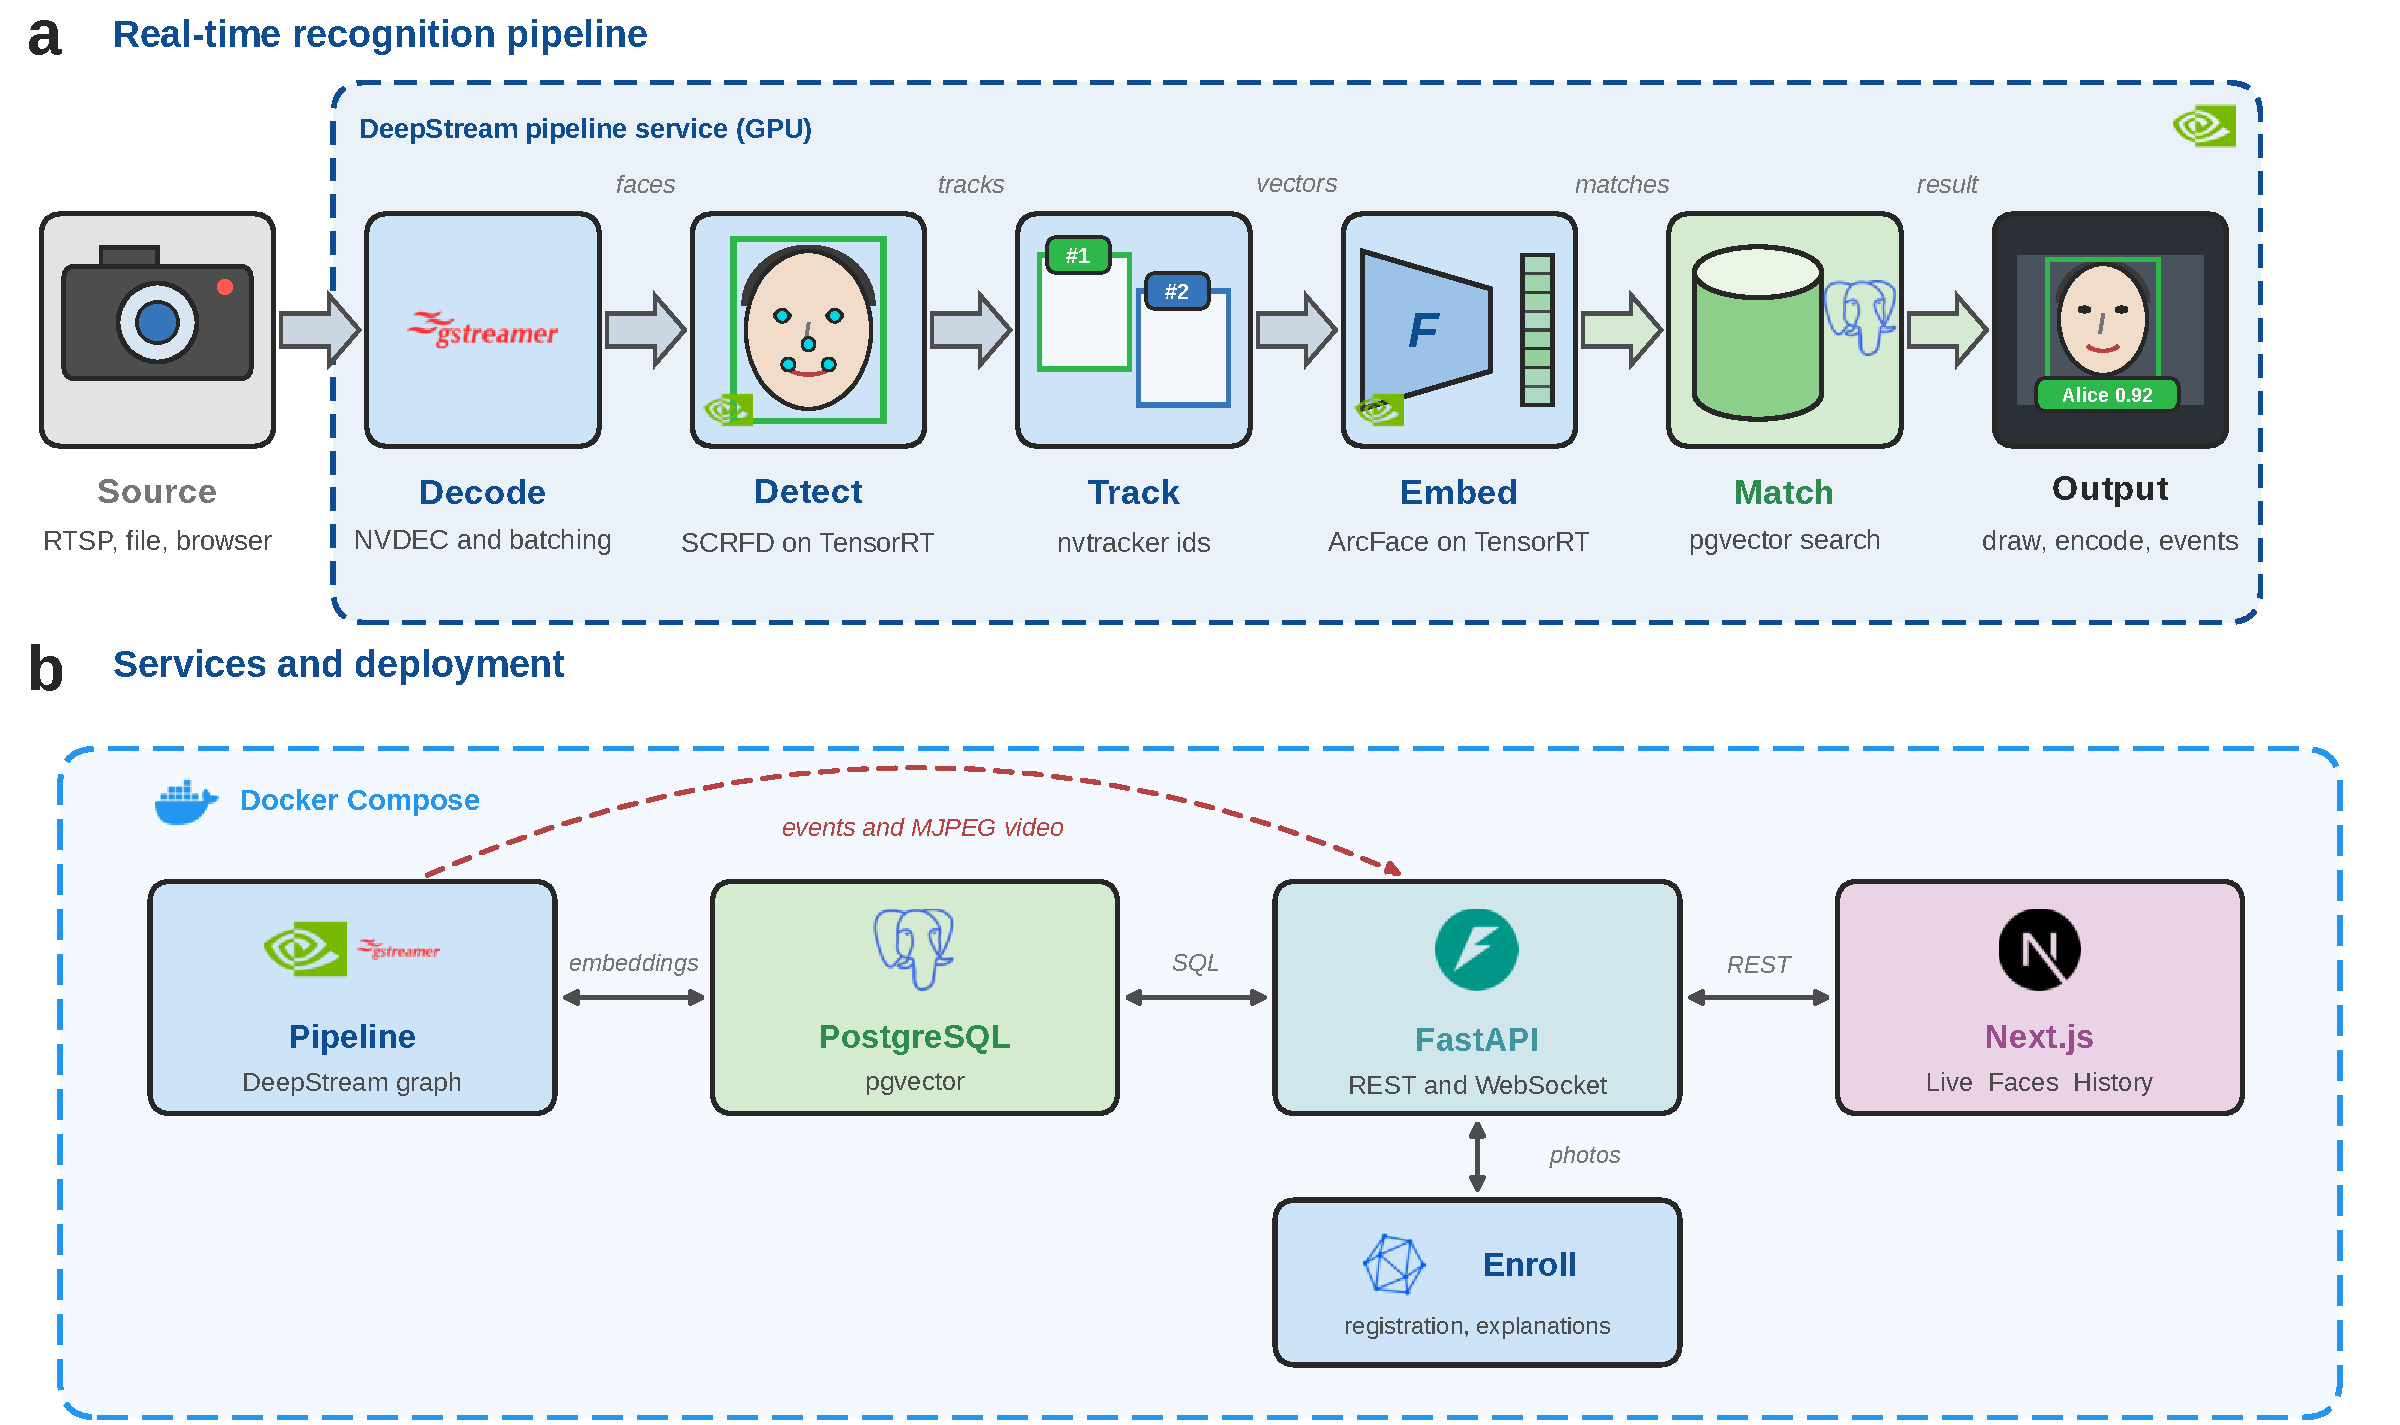
\includegraphics[width=0.92\linewidth]{figures/architecture.pdf}
  \caption{Recognition pipeline (a) and the services that deliver it (b).}
\end{figure}

% ================================================================ III. Quick Start
\newpage
\section{Quick Start}
You need Docker with Compose v2, an NVIDIA GPU (DeepStream runs on the GPU), and a camera or an RTSP stream.
Clone the repository, then start the services.
\begin{terminal}{Terminal}
git clone https://github.com/hugebenevolence/face_recognized_system.git
cd face_recognized_system
docker compose --profile sim up --build
\end{terminal}
Once the services are healthy, open \href{http://localhost:3000}{\texttt{http://localhost:3000}}.
The first start also builds the TensorRT engines, which takes a few minutes.

% ================================================================ IV. Using the system
\section{Using the System}

\subsection{Register a person}
\noindent\begin{minipage}[c]{0.62\linewidth}
  \begin{itemize}
    \item Open \textbf{Faces}, then enter a name and an ID.
    \item Add photos with \textbf{Open camera}, by upload, or from a \textbf{Group photo}.
    \item Review the report. Not only does it grade each photo, but it also estimates how easily the person could be confused with others.
  \end{itemize}
\end{minipage}\hfill
\begin{minipage}[c]{0.34\linewidth}
  \shot{figures/ui_register.png}{Faces page: registration form and people list}
\end{minipage}

\subsection{Recognize live}
\noindent\begin{minipage}[c]{0.34\linewidth}
  \shot{figures/ui_live.png}{Live page: camera picker, video, and events}
\end{minipage}\hfill
\begin{minipage}[c]{0.62\linewidth}
  \begin{itemize}
    \item Open \textbf{Live} and choose a camera. Webcams, RTSP streams, and video files are supported.
    \item Known people appear with a green box and a score. Anyone else is labeled \emph{Unknown}.
    \item Switch on \textbf{Explain overlay} to display the landmarks and the decision scores.
  \end{itemize}
\end{minipage}

\subsection{Review the history}
\noindent\begin{minipage}[c]{0.62\linewidth}
  \begin{itemize}
    \item Open \textbf{History} to search by person and to filter by status or time.
    \item Select \textbf{Why} on any row to inspect the evidence behind that decision.
    \item Use \textbf{Explain regions} to see which parts of the face influenced the score.
  \end{itemize}
\end{minipage}\hfill
\begin{minipage}[c]{0.34\linewidth}
  \shot{figures/ui_history.png}{History page: filters and recognition log}
\end{minipage}

\begin{callout}{aiopurple}{\faLightbulb}{Tips}
\begin{itemize}
  \item Should recognition feel unreliable, add two or three photos taken with the same camera and lighting.
  \item Should the video stay blank, confirm the camera on \textbf{Live}, then run \texttt{docker compose ps}.
  \item Without a camera, put a video in \texttt{samples} and add \texttt{-{}-profile sim} to the start command.
\end{itemize}
\end{callout}

\end{document}
